\documentclass[conference]{IEEEtran}
\usepackage[top=0.5in]{geometry} 
\usepackage{graphicx} 
\usepackage{hyperref}
\usepackage{amsmath}

\title{CS/CE 412/471 Project Report \\ Randomised Heap Exploration}
\author{Musab Kasbati, Meesum Abbas}
\date{}

\begin{document}

\maketitle

\section{Background and Motivation}

The \textit{explorable heap selection problem} concerns selecting the $n$-th smallest element in a binary heap where values can only be accessed through traversal from the root. Each move across an edge incurs a unit cost, making total distance traveled the primary complexity measure. Originally proposed by Karp, Saks, and Wigderson \cite{karp1986search}, this model captures challenges faced by branch-and-bound algorithms operating under memory constraints.

Prior to this work, randomized algorithms for explorable heap selection exhibited a runtime barrier of $n \cdot \exp(O(\sqrt{\log n}))$ with a memory usage of $O(\sqrt{\log n})$, leaving substantial room for improvement. This problem is not merely of theoretical interest: efficient traversal strategies can significantly accelerate memory-constrained search procedures used in optimization tasks like integer programming (e.g., MIP solvers). Since many combinatorial optimization problems can be modelled as integer programs (such as 0-1 knapsack, graph-coloring, travelling salesman), optimizations to branch and bound can have significant impacts on real-world optimization tasks. Even when memory is abundant, emphasizing locality and minimizing tree traversal costs remain critical for performance when computation for neighbouring nodes overlap. 

This paper introduces a nearly optimal randomized algorithm that dramatically reduces the expected runtime to $O(n \log^3 n)$ using $O(\log n)$ space. Moreover, a theoretical lower bound of $\Omega(\frac{n \log(n)}{\log(\log (n)})$ runtime for $O(\log n)$ space is also proven. These results represent a substantial theoretical advancement with tangible implications for real-world optimization, resource allocation, and routing problems where efficient tree search is vital.

\section{Algorithmic Description}

The algorithm operates on an infinite binary (min-)heap and, given a target rank $n$, outputs the $n$-th smallest element. The key idea is to progressively find all $n$ smallest elements through controlled exploration, using randomness and recursion to minimize the search cost.

Initially, the algorithm starts with a subtree consisting solely of the root (the overall smallest element). It then repeatedly doubles the size of this subtree by expanding it through its immediate descendants until the subtree contains $n$ nodes. Throughout this process, an important invariant is maintained: all nodes in the selected subtree must be \textit{good}.

A node is considered \textit{good} if its value is less than the true $n$-th smallest element. Although this threshold is unknown in advance, goodness can be determined using a depth-first search (DFS). Given a candidate value, the DFS explores the heap from the root, only following nodes with smaller values. If the search visits at most $n$ nodes, the candidate is \textit{good}; otherwise, if more than $n$ smaller nodes are encountered, it is deemed \textit{bad}. The min-heap property guarantees that once a node with a larger value is found, all its descendants are also larger, allowing efficient pruning of the search.

In parallel, the algorithm maintains a dynamic range $(\mathcal{L}, \mathcal{U})$, where $\mathcal{L}$ and $\mathcal{U}$ respectively represent lower and upper bounds on the $k$-th smallest element, with $k$ tracking the current subtree size. Initially, $\mathcal{L}$ is set to the root's value and $\mathcal{U}$ is set to $+\infty$. This range is refined as exploration proceeds.

Whenever the subtree needs to expand, the algorithm selects a random unselected subtree to explore, which has a node value that falls within the current range $(\mathcal{L}, \mathcal{U})$. It then recursively applies the same strategy to this subtree to find the additional \textit{good} nodes required. Importantly, since the heap is infinite, any subtree will have enough nodes to satisfy this requirement.

Within each such recursive step, the algorithm effectively performs a binary search within the subtree: it samples node values to identify the largest \textit{good} value ($\tilde{\mathcal{L}}$) and the smallest \textit{bad} value ($\tilde{\mathcal{U}}$). These values are then used to tighten the global range:
\[
\mathcal{L} \leftarrow \max(\mathcal{L}, \tilde{\mathcal{L}}), \quad \mathcal{U} \leftarrow \min(\mathcal{U}, \tilde{\mathcal{U}}).
\]
By repeatedly halving the number of candidates with each iteration, the algorithm ensures rapid convergence to a single value $\mathcal{V}$, which matches the $k$-th smallest element.

As $k$ is doubled in each expansion phase, the algorithm quickly reaches $k = n$, thereby identifying the $n$-th smallest element of the original heap. This approach achieves an expected time complexity of $O(n \log^3 n)$ while using only $O(\log n)$ space.


\section{Implementation Summary}

We implemented the full \textsc{RandomisedHeapExploration} algorithm as described in \cite{Borst2025}, alongside a simpler baseline algorithm for verification and runtime benchmarking. We further applied the algorithm to a practical problem: solving integer linear programs, specifically the 0-1 Knapsack problem. 

The major components of our implementation are as follows:

\begin{enumerate}
    \item \textbf{Infinite Heap Construction:} We designed a heap structure where nodes are generated dynamically as they are accessed, enforcing a parent-first exploration order consistent with the explorable heap setting. We implemented three types of heaps:
    \begin{itemize}
        \item \textsc{firstN}: The root is labelled as $1.0$. Moreover, for a node with value $k$, its left and right child have values $2k$, $2k+1$, respectively. Effectively, a BFS flattened version of the heap would give the values $1, 2, 3, \ldots$
        \item \textsc{randGen}: Nodes with random values while preserving the heap property. Values may repeat.
        \item \textsc{knapsack}: Nodes representing solutions to subproblems of a linear programming relaxation of the 0-1 Knapsack problem. The traversal at level $i$ of either left or right enforces a constraint of 0 or 1, respectively, on the $i$-th item.
    \end{itemize}
    
    \item \textbf{Algorithm Implementation:} We fully implemented the \textsc{RandomisedHeapExploration} algorithm and its core subroutines, including \textsc{Select}, \textsc{Extend}, \textsc{Roots}, \textsc{DFS}, and \textsc{GoodValues}. While pseudocode for \textsc{Select} and \textsc{Extend} was provided in the paper, the other subroutines were implemented based on their described behavior.
    
    \item \textbf{Baseline Algorithm:} We implemented a simpler \textsc{BestFirst} algorithm that greedily explores the node with the smallest known value. Although it uses significantly more memory, it provides a practical tool for verifying the correctness of our main implementation and for runtime comparisons.
    
    \item \textbf{Application to Optimization:} We applied the \textsc{RandomisedHeapExploration} algorithm within a Branch-and-Bound framework to solve integer linear programs arising from instances of the 0-1 Knapsack problem.
    
    \item \textbf{Visualization Tools:} To aid understanding and debugging, we developed a visualization system that animates the execution of the algorithm, highlighting node status depending on the caller of \textsc{Extend}, emphasizing selected roots, and concealing nodes identified as \textit{bad}.
\end{enumerate}

\subsection*{Implementation Strategy and Challenges}

Our implementation strategy was to modularize the project, with clear separations between heap generation, core algorithm subroutines, baseline comparison, and the application to integer programming. This structure allowed for easier testing, debugging, and future extensibility to different types of heaps or problem domains.

\textbf{Infinite Heap Implementation:}  
Creating an infinite heap was a nontrivial task. We achieved this by breaking down the heap structure into classes and designing wrapper functions for child access. Instead of pre-creating the entire tree, child nodes were dynamically generated upon access, creating the illusion of an infinite structure while preserving strict parent-first accessibility.

\textbf{Subroutines Without Pseudocode:}  
A significant challenge was the absence of pseudocode for key subroutines (\textsc{Roots}, \textsc{DFS}, and \textsc{GoodValues}), requiring careful, line-by-line interpretation of their described behaviors. Furthermore, the description of \textsc{GoodValues} appeared to have an inconsistency: if all nodes were "good," the random binary search would fail. We resolved this by adding an initial check for the largest value before starting the search.

\textbf{Handling Duplicate Values:}  
The original algorithm assumes distinct values in the heap, but when applying the method to 0-1 Knapsack problems, duplicate values naturally arise. To accommodate this, we modified \textsc{DFS}: instead of checking whether there are at most $n$ values less than the current threshold $L$, we checked whether the $n$-th largest value was at most $L$. This subtle adjustment was critical to maintaining correctness.

\textbf{Adapting for Integer Linear Programming:}  
Applying the algorithm to integer linear programming was itself a challenge. The original paper’s description of this step was abstract, and we supplemented our understanding by consulting \cite{karp1986search}. Even then, practical details were missing, so we studied linear programming, integer programming, and the Branch-and-Bound method independently to understand how the 0-1 Knapsack problem could be formulated and solved within this framework. This was a fascinating deep dive and substantially enriched our understanding of the broader algorithmic context.

\textbf{Visualization Challenges:}  
Building a meaningful visualization required a deep understanding of the algorithm's internal dynamics. We worked to highlight important steps, such as node classification based on the caller of \textsc{Extend}, selection of roots, and hiding of "bad" nodes. However, creating an intuitive visualization remained challenging—especially for first-time viewers unfamiliar with the algorithm’s recursive structure.

Overall, while the core implementation faithfully follows the original algorithmic design, we made thoughtful adaptations where necessary and developed auxiliary tools for verification and insight.

\section{Evaluation}

\subsection{Base Algorithm Correctness Testing}

To validate the correctness of the implemented algorithm, we conducted extensive testing in controlled as well as randomized settings.

First, we tested the algorithm on the \textsc{firstN} heap structure, where nodes are simply the integers $1, 2, 3, \ldots$. As expected, the algorithm correctly identified the $n$-th smallest element as $n$ itself, verifying basic functionality on a predictable structure.

Next, we moved to more complex scenarios using randomly generated heaps (\textsc{randGen}). For small values of $n$, we verified correctness manually by drawing the heap and comparing the output value with a manual verification (see Figures \ref{fig:visualise} and \ref{fig:result}). 

For larger values of $n$, we conducted stress tests on 50 randomly generated heaps with $n \in [100, 50000)$. In each case, the final result was compared to the output produced by the baseline \textsc{BestFirst} algorithm. The randomized heap exploration algorithm consistently returned correct results, demonstrating its robustness across a wide range of input sizes and structures.

\begin{figure}
    \centering
    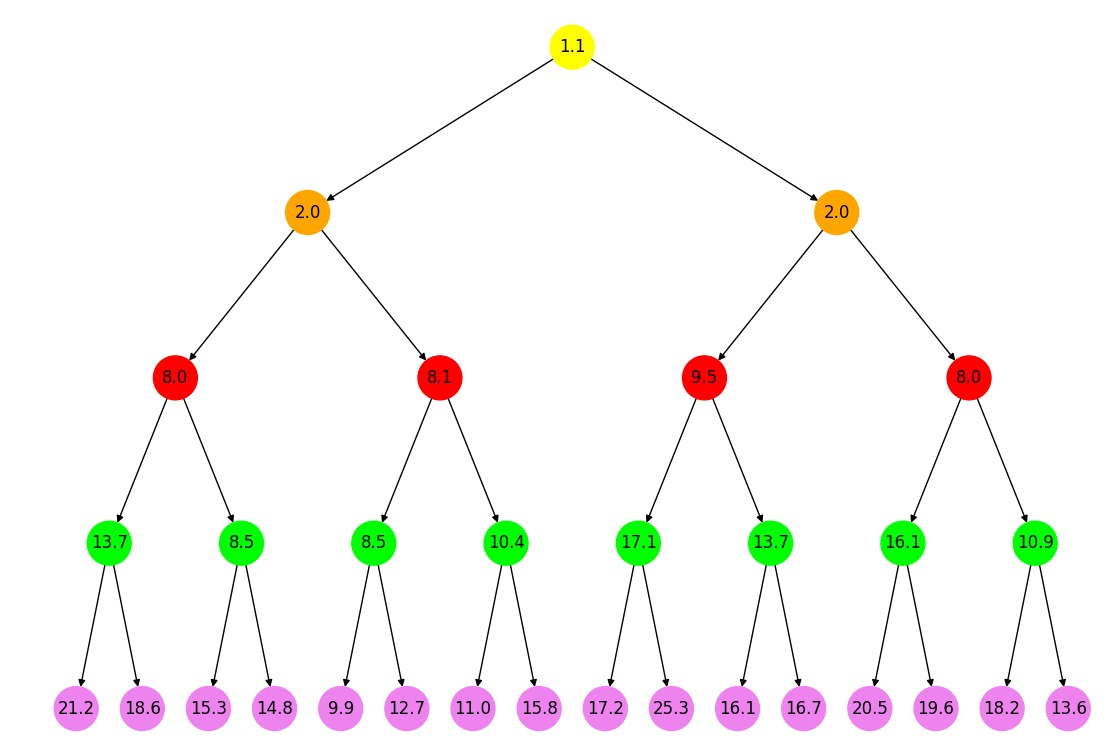
\includegraphics[width=1\linewidth]{images/algo-visualisation.jpeg}
    \caption{Visualization of heap search algorithm with $n = 8$}
    \label{fig:visualise}
\end{figure}

\begin{figure}
    \centering
    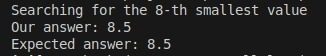
\includegraphics[width=1\linewidth]{images/algo-result.jpeg}
    \caption{Results of heap search algorithm with $n = 8$}
    \label{fig:result}
\end{figure}


\subsection{Base Algorithm Complexity \& Runtime Analysis}

The theoretical time complexity of the randomized heap exploration algorithm, as stated in the original paper, is $O(n \log^3 n)$. To empirically verify this, we measured the runtime of our implementation across various values of $n$ and normalized it by different complexity estimates.

The normalized plots (Figure \ref{fig:normailsed-run-time}) suggest that the observed runtime actually grows somewhat slower than $O(n \log^3 n)$ and is closer to $O(n \log n)$ for randomly generated heaps. This discrepancy is expected: the worst-case complexity may not have been realized in our randomly generated test cases, and random heaps may have more favorable structural properties compared to worst-case constructed heaps.

Thus, while our experiments confirm that the theoretical upper bound holds for our tested inputs, the practical performance may be better than the worst-case analysis would suggest.

\begin{figure}
    \centering
    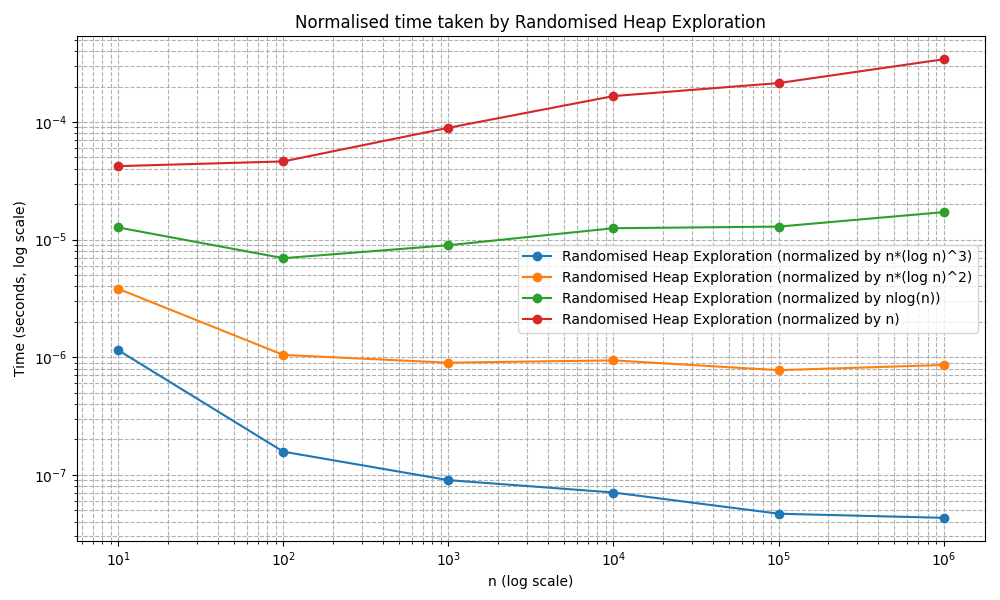
\includegraphics[width=1\linewidth]{images/algo-complexity.png}
    \caption{Normalized running times (log-scale)}
    \label{fig:normailsed-run-time}
\end{figure}

\subsection{Comparative Evaluation against Baseline Algorithm}

We compared the randomized heap exploration algorithm to the baseline \textsc{BestFirst} algorithm, which explores nodes in a best-first manner based on their value. As shown in Figure \ref{fig:comparison}, the randomized approach has a slightly higher runtime compared to \textsc{BestFirst}. 

This outcome is consistent with the theoretical expectations: the randomized algorithm trades off a slightly worse time complexity ($O(n \log^3 n)$) to achieve significantly better space efficiency ($O(\log n)$) compared to \textsc{BestFirst}'s $O(n)$ space complexity with $O(n \log n)$ runtime. 

Despite the slight increase in runtime, the randomized heap exploration algorithm maintains correctness and offers substantial memory savings, making it a better choice in memory-constrained environments. Importantly, across all tested instances, both algorithms produced matching results.

\begin{figure}
    \centering
    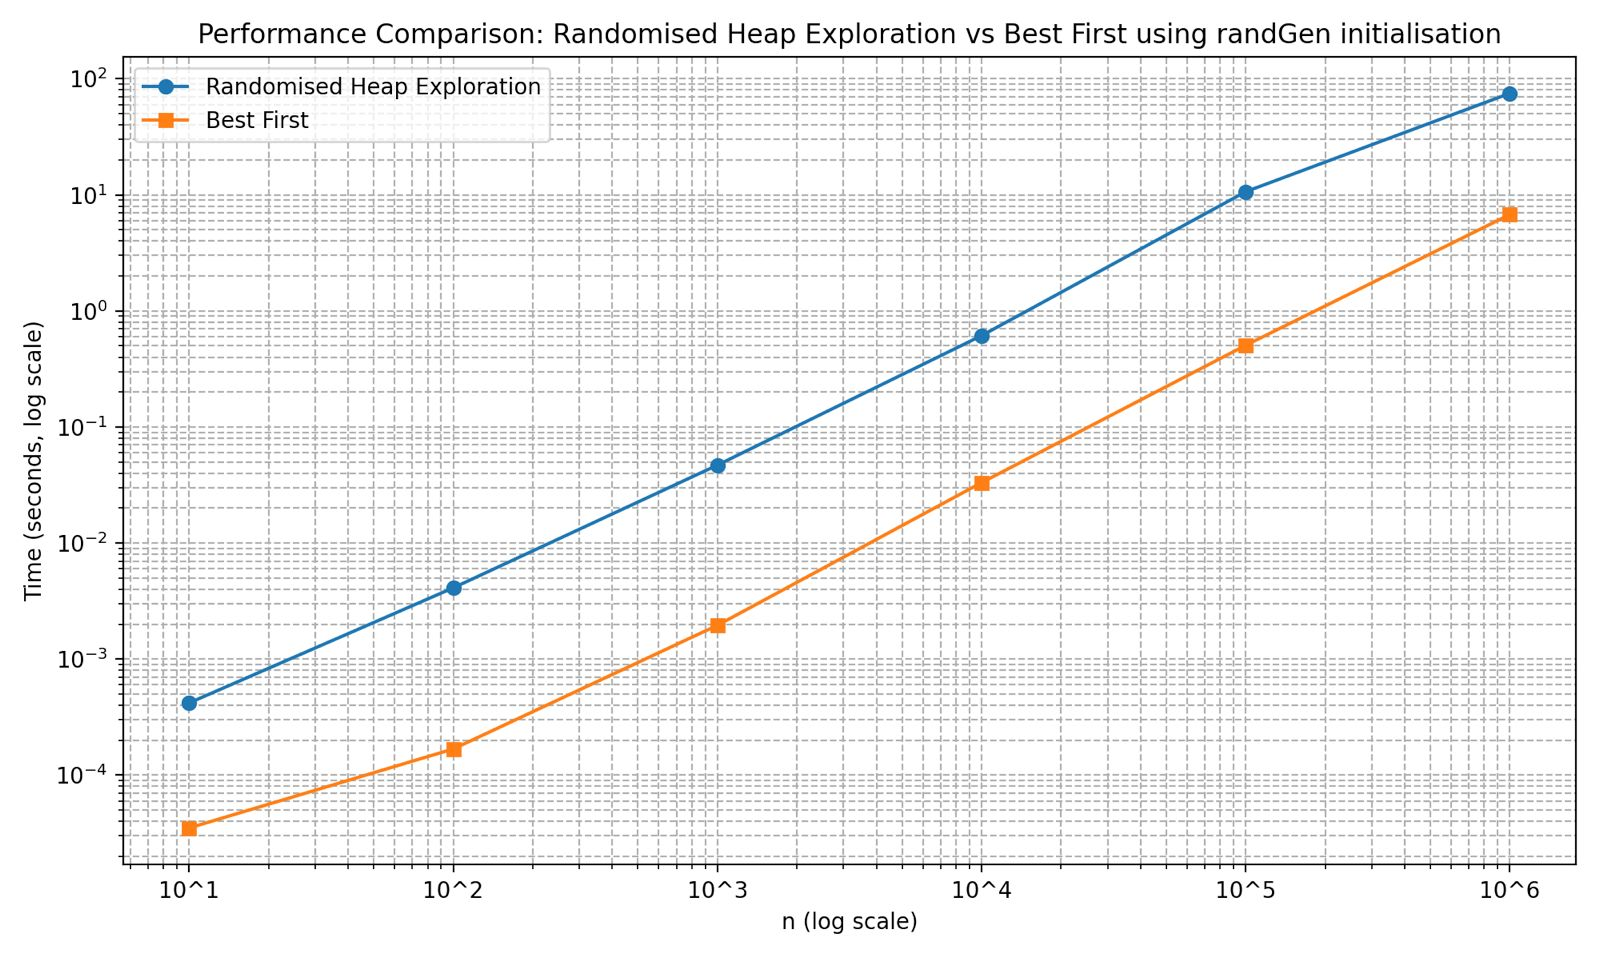
\includegraphics[width=1\linewidth]{images/algo-comparison.jpeg}
    \caption{Baseline (\textsc{BestFirst}) vs Randomized Heap Exploration runtime comparison}
    \label{fig:comparison}
\end{figure}

\subsection{0-1 Knapsack Correctness Testing}

To test the correctness of our application of the randomized heap exploration algorithm to solving 0-1 Knapsack problems via branch and bound, we adopted the following approach:

We constructed a heap where each node represents the negative (for min-heap property) value of a solution to a relaxed (linear programming) knapsack problem. We searched for the $k$-th smallest value in the heap, doubling $k$ progressively (starting from 1) until a terminal node—corresponding to an integer (0-1) solution—was discovered during exploration. After identifying the existence of some terminal node, we selected the smallest negative terminal value by constraining our heap traversal by the $k$-th value limit identified by the heap exploration. This allowed us to efficiently isolate optimal integer solutions. The negative of this value represented the optimal value, while the edge traversals from root (left = 0, right = 1) determine the solution. 

\vspace{0.5em}
\noindent
\textbf{Datasets Used:}
We tested the algorithm on the following two instances:

\begin{itemize}
    \item \textbf{Small Instance:}  \\
    Weights = [12, 7, 11, 8, 9],  \\
    Prices = [24, 13, 23, 15, 16],  \\
    Knapsack Capacity = 26 \\
    Optimal Value = 51.0 \\
    Optimal Solution = [0, 1, 1, 1, 0] \\
    \item \textbf{Medium Instance:}  \\
    Weights = [23, 31, 29, 44, 53, 38, 63, 85, 89, 82], \\  
    Prices = [92, 57, 49, 68, 60, 43, 67, 84, 87, 72], \\
    Knapsack Capacity = 165 \\
    Optimal Value = 309.0 \\
    Optimal Solution = [1, 1, 1, 1, 0, 1, 0, 0, 0, 0] \\
\end{itemize}

\vspace{0.5em}
\noindent
\textbf{Verification:}
The correctness of the algorithm’s output was verified by comparing the results against the solutions obtained using the \texttt{PuLP} library's integer linear programming solver. In both the small and medium instances, the solutions produced by our heap exploration approach matched the exact solutions provided by the solver, thereby confirming the correctness of our implementation.


\section{Enhancements}

To extend and deepen the original implementation, we introduced several enhancements that not only improved the algorithm's applicability and robustness but also provided better insight into its working:

\begin{enumerate}
    \item \textbf{Confirming Correctness Empirically through Testing on Randomly Generated Data:}  
    We created a variety of randomly generated heaps to stress-test the algorithm under diverse scenarios. This helped verify the algorithm's correctness across different heap structures and node distributions, increasing our confidence in its general robustness.

    \item \textbf{Correcting the \textsc{GoodValues} Subroutine:}  
    During implementation, we discovered that the description of the \textsc{GoodValues} procedure had a flaw: if all candidate values were "good," the randomized binary search could fail. We resolved this by adding an initial check for the largest value before proceeding with binary search. This correction improved the stability and reliability of the algorithm, particularly for edge cases where most nodes satisfy the target condition.

    \item \textbf{Supporting Repeated Values in Nodes:}  
    The original design assumed all heap node values were distinct. However, many practical applications, such as variants of the Knapsack problem, naturally involve repeated values. We modified the \textsc{DFS} subroutine to handle repeated values by adjusting the comparison logic: instead of ensuring at most $n$ nodes are $\leq L$, we check if the $n$-th largest value is $\leq L$. This subtle but important modification significantly broadened the algorithm's applicability to real-world scenarios.

    \item \textbf{Application to 0-1 Knapsack via Branch and Bound:}  
    We explored using the heap exploration algorithm within a branch-and-bound framework for solving 0-1 Knapsack problems. By framing the search space as an explorable heap and combining it with integer linear programming ideas, we demonstrated that the algorithm could contribute to solving a classical optimization problem. This extension highlighted the versatility of the method beyond pure heap search tasks.

    \item \textbf{Development of a Visualization Tool:}  
    To better understand and communicate the algorithm's behavior, we developed a custom visualization tool. It animates node exploration, pruning, and root selection steps, offering an intuitive window into the algorithm's internal workings. Creating the visualization required a deep dive into each subroutine and helped us identify areas of optimization and debugging more effectively. Although the visualization remains somewhat complex for first-time viewers, it proved invaluable for internal validation and understanding.
\end{enumerate}

\vspace{0.5em}
\noindent
\textbf{Impact and Motivation:}  
These enhancements were motivated by a desire to rigorously test the algorithm's boundaries, fix ambiguities in the original description, adapt the algorithm to more realistic settings, and make the internal process transparent through visualization. Collectively, these improvements resulted in a more robust, flexible, and insightful implementation, demonstrating the algorithm’s potential for broader applications.

\section{Reflection}

One of the key challenges faced during this project was navigating dense theoretical text. Understanding the randomized heap exploration algorithm, along with its application to integer programming, required carefully working through technical descriptions and learning to explore new problem domains such as linear programming. This process taught us how to leverage multiple resources—research papers, online lectures, articles—to build a coherent understanding of unfamiliar topics.

Another important learning was how to structure code modularly. By separating concerns into independent modules (heap generation, algorithm subroutines, visualization, applications), we were able to make the codebase much easier to debug, extend, and maintain. Additionally, we realized the importance of taking a layered approach to problem-solving: building a fuller conceptual picture first before diving into implementation saved time and reduced mistakes later on.

The main learning outcomes from this project included:
\begin{itemize}
    \item Gaining an appreciation for the power of randomization in algorithm design.
    \item Understanding the fundamentals of linear programming and the branch and bound method for solving integer programs.
    \item Developing skills in reading and interpreting research papers, including dealing with ambiguities or missing details.
\end{itemize}

For future work, several directions seem promising. One is developing methods to better handle heaps filled with identical values (as opposed to just occasional duplicates), where the current approach may not be efficient. Another is expanding the visualization: by adding finer-grained highlights, step-by-step captions, or dynamic explanations during the animation, we could make the algorithm much more accessible to people encountering it for the first time.

Overall, this project provided valuable experience not just in implementing a complex algorithm, but also in the broader skills required for tackling research-level problems: exploration, abstraction, and critical thinking.

\bibliography{references}
\bibliographystyle{plain}

\end{document}
